% CHAPTER 1
\chapter{VALIDATION IN TEST CASE}
\label{chp:4}
\section{P.M.Anderson 9 Bus Test Case}
\subsection{System Properties}
In order to understand frequency dynamics better, P.M. Anderson test case has been used in the study. The single line diagram of the system is given in Figure \ref{ieee_9_bus}. The test case consists of three generators and three loads. Generators in the system are connected to 230 kV high voltage network with transformers.\par
\begin{figure}[h!]
	\centering
	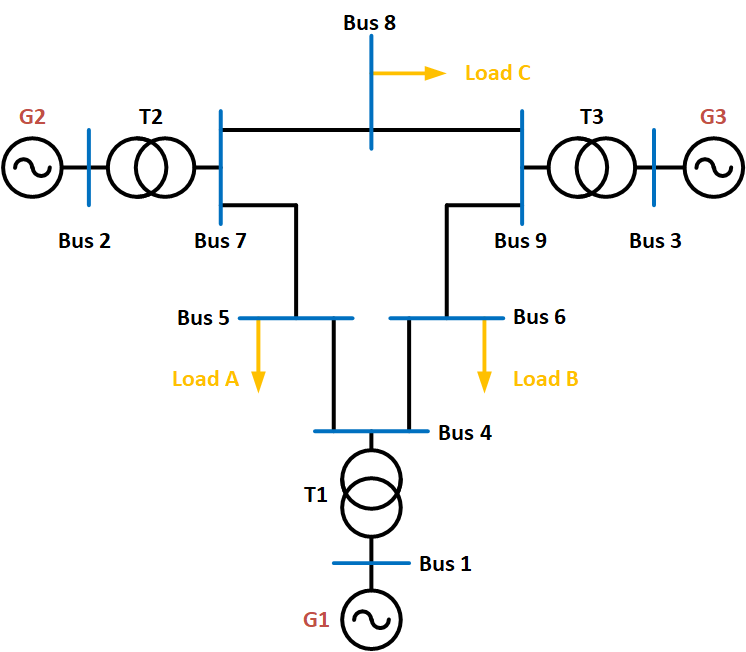
\includegraphics[width=.85\linewidth]{ieee_9_bus.png}
	\caption{P.M.Anderson Test Case}
	\label{ieee_9_bus}
\end{figure}
The biggest generator in the system is a hydropower plant with a power rating of 247.5 MVA. The remaining ones are steam generators. The power ratings of the generators are given in Table \ref{generatorproperties}.\par
\begin{table}[h!]
	\centering
	\begin{tabular}{ccc}
		\hline
		\textbf{Generators} & \textbf{Power Rating (MVA)} & \textbf{Plant Type} \\ \hline
		Gen 1               & 247.5                       & Hydro				\\
		Gen 2               & 192                         & Steam               \\
		Gen 3               & 128                         & Steam               \\ \hline
	\end{tabular}
	\caption{Generator Properties of Test System}
	\label{generatorproperties}
\end{table}
The loads in the system are connected directly to the high voltage network. The active and reactive power ratings of the loads are listed in Table \ref{loadproperties}.
\begin{table}[h!]
	\centering
	\begin{tabular}{ccc}
		\hline
		\textbf{Generators} & \textbf{Active Power (MW)}  & \textbf{Reactive Power (MVAr)} \\ \hline
		Load A              & 125                      	  & 50				 \\
		Load B              & 90                          & 30                \\
		Load C              & 100                         & 35                \\ \hline
	\end{tabular}
	\caption{Load Properties of Test System}
	\label{loadproperties}
\end{table}
\subsection{Load Flow Analysis}
Successful grid operation requires a load flow analysis in order to ensure that bus voltages are inside the allowed band and power flows are below the power carrying capabilities of the lines. Load flow results are given in Table \ref{loadflow}.
\begin{table}[h!]
	\centering
	\begin{tabular}{cclccccc}
		\hline
		\textbf{Bus \#} & \textbf{Type} & \multicolumn{1}{c}{\textbf{Voltage}} & \textbf{Angle} & \textbf{Pg} & \textbf{Qg} & \textbf{Pl} & \textbf{Ql} \\ \hline
		1               & SL            & \multicolumn{1}{c}{1.04}             & 0              & 70.8        & 20.91       & 0           & 0           \\
		2               & PV            & \multicolumn{1}{c}{1.025}            & 9.4            & 163         & 12.42       & 0           & 0           \\
		3               & PV            & \multicolumn{1}{c}{1.025}            & 4.72           & 85          & -10.16      & 0           & 0           \\
		4               & PQ            & 1.0293                               & -2.18          & 0           & 0           & 0           & 0           \\
		5               & PQ            & 1.0057                               & -3.89          & 0           & 0           & 125         & 50          \\
		6               & PQ            & 1.0149                               & -3.63          & 0           & 0           & 90          & 30          \\
		7               & PQ            & 1.0224                               & 3.83           & 0           & 0           & 0           & 0           \\
		8               & PQ            & 1.0137                               & 0.8            & 0           & 0           & 100         & 35          \\
		9               & PQ            & 1.0320                               & 2.03           & 0           & 0           & 0           & 0           \\ \hline
	\end{tabular}
	\caption{Load Flow Results in Base Case}
	\label{loadflow}
\end{table}